	\subsection{Sous-mission A4}

	\begin{vwcol}[widths={0.65,0.2}, rule=0pt]
	\begin{minipage}{0.7\textwidth}
	\paragraph{Objectifs de la mission}

	Rendre une image de la planète Jupiter plus nette. Pour se faire nous avions à disposition deux photographies faites à quelques secondes d'intervalle comprenant toutes deux du bruit.
	\end{minipage}

	\begin{minipage}{0.3\textwidth}
	\begin{flushright}
	\paragraph{Techniques utilisés}

	Soustraction \& Filtre médian
	\end{flushright}
	\end{minipage}

	\end{vwcol} 

	\begin{figure}[h]
	\centering
		\begin{multicols}{2}
		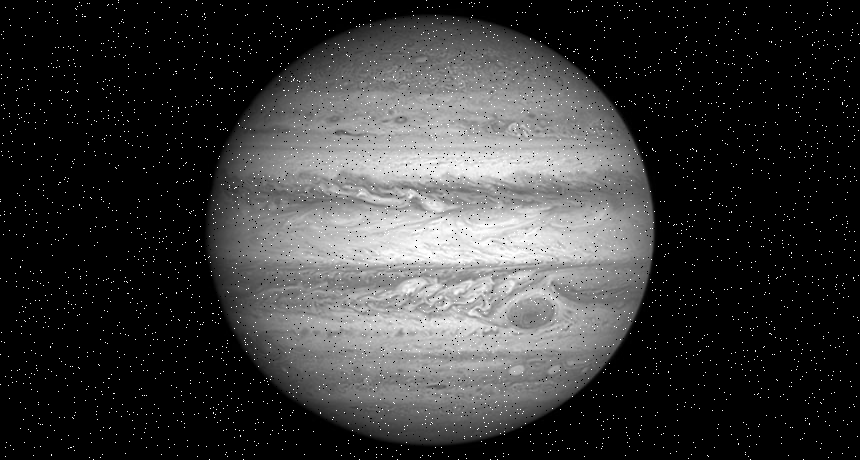
\includegraphics[scale=0.325]{images/Jupiter.png}
		Avant
		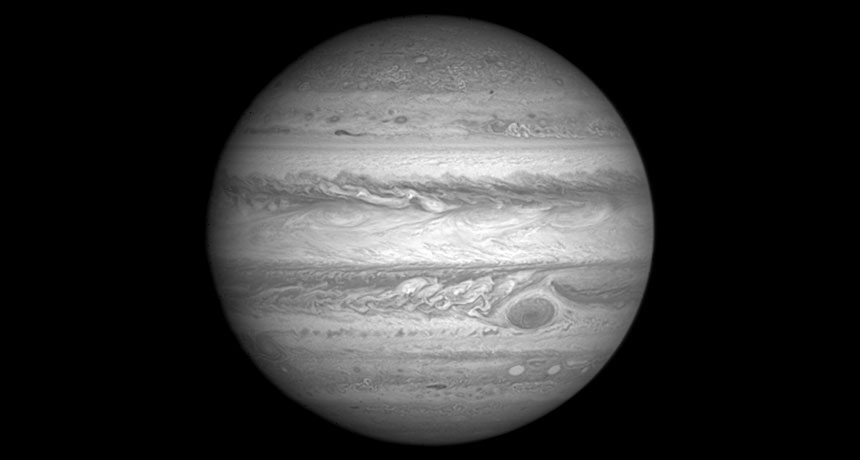
\includegraphics[scale=0.325]{images/JupiterAp.png}
		Après
		\end{multicols}
	\end{figure}
	\vspace{-0.9cm}

	\paragraph{Procédé}	
		Le résultat ci-dessus, nous avons utilisé deux filtes à la suite. Tout d'abord, nous avons \emph{soustrait} les deux images ensembles pour obtenir une troisième image ne comprenant que le bruit. Nous avons alors \emph{soustrait} ce résultat a l'image d'origine. Nous obtenons ensuite une image de meilleure qualité mais tout de même bruitée. Pour résoudre ce problème nous avons utilisé un \emph{filtre médiant} permettant de retirer le bruit sans altérer la netteté de l'image.